\textit{Solución.} A continuación, se muestran las curvas obtenidas a partir de la ecuación característica para distintos valores de la perturbación $X _{vs} (t)$.

\begin{figure}[!h]
    \centering
    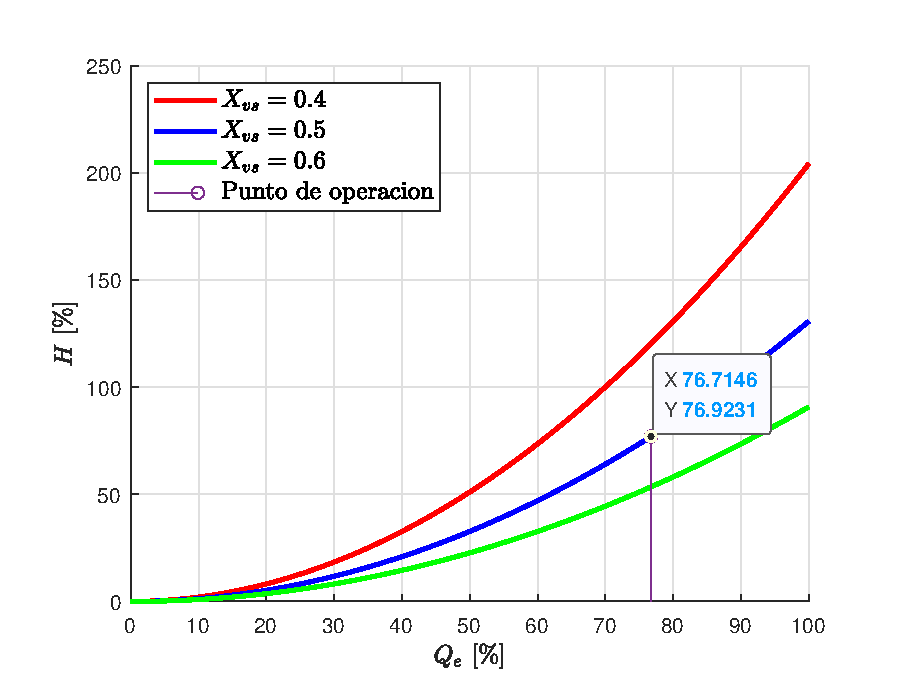
\includegraphics[width = 0.5\linewidth]{figs/fig6.eps}
    \caption{Curva estática del proceso para los distintos valores del pocentaje de apertura de la válvula de salida $X _{vs} (t)$}
    \label{fig5}
\end{figure}

Note que el punto de operación se encuentra en el valor central de $X _{vs} (t)$, ya que este fue el valor que se tomó en cuenta para el cálculo del punto de operación, así como para generar el modelo linealizado.

